% Provenance (never printed): see sources/outline_sources.md (Year 1:
% geological cross-sections, apparent dip, thickness, boreholes). Every
% Varden Hills number comes from figdata/bachelor-1/varden_sections.py, which
% imports the shared model figdata/shared/region.py; numbers of the exercises
% and problem in the Book 3 scratch calculator and in that script's values.
\chapter{Seções geológicas}\label{ch:b1:cross-sections}

Uma empresa de engenharia planeja um túnel sob as Colinas de Varden, em linha reta de oeste para leste, em uma altitude constante de \qty{200}{m}. Antes que se perfure um único metro, os geólogos precisam dizer quais rochas a máquina vai cortar, onde ela cruzará a falha e quanto tempo passará no calcário, uma rocha que pode conter cavidades abertas e água. Ninguém consegue ver o interior das colinas; mas o \omterm{def:b1:geological-maps:geological-map}{mapa geológico} de \cref{ch:b1:geological-maps}, algumas sondagens e a geometria dos planos bastam para desenhar uma fatia vertical do terreno --- uma \omterm{def:b1:cross-sections:section}{seção geológica} --- e para ler as respostas nela. Este capítulo ensina como uma seção é construída a partir de um mapa, como \omterm{def:b1:geological-maps:attitude}{mergulhos} e espessuras mudam quando a fatia é cortada obliquamente, como as sondagens são correlacionadas e como uma seção conta a história das rochas que corta. Ele termina com o túnel.

\begin{recall}
A \omterm{def:b1:geological-maps:attitude}{atitude} de um plano é dada pelo seu \omterm{def:b1:geological-maps:attitude}{sentido de mergulho} $\alpha$ e pelo seu \omterm{def:b1:geological-maps:attitude}{mergulho} $\delta$, e o plano que passa por um ponto de altitude $z_0$ na origem é $z = z_0 - \tan\delta\,(x\sin\alpha + y\cos\alpha)$; três pontos de um contato fixam a sua \omterm{def:b1:geological-maps:attitude}{atitude}; a regra do V lê o \omterm{def:b1:geological-maps:attitude}{mergulho} a partir do padrão dos \omterm{def:b1:geological-maps:geological-map}{afloramentos} em vales (\cref{ch:b1:geological-maps}). Uma curva de nível une pontos de mesma altitude em um mapa topográfico (Livro 1, 9º ano). Rochas mais novas repousam sobre as mais antigas, e o que corta uma rocha é mais novo que ela (Livro 1, 7º ano).
\end{recall}

\section{Do mapa à seção}

\begin{definition}[Seção geológica, perfil topográfico, exagero vertical]\label{def:b1:cross-sections:section}
Uma \emph{seção geológica}\index{seção geológica} é um desenho das unidades rochosas e das estruturas em um plano vertical através do terreno, ao longo de uma linha traçada no mapa. Sua borda superior é o \emph{perfil topográfico}\index{perfil topográfico}, a curva da altitude do terreno ao longo da linha. O \emph{exagero vertical}\index{exagero vertical} $e$ de uma seção é a razão entre a sua escala vertical e a sua escala horizontal; a seção está em \emph{escala verdadeira} quando $e = 1$.
\end{definition}

\begin{method}[Construção de uma seção geológica a partir de um mapa]\label{met:b1:cross-sections:construct}
\begin{enumerate}
  \item Trace a linha de seção no mapa e apoie a borda de uma tira de papel sobre ela; marque onde cada curva de nível a cruza, com a sua altitude, e onde cada contato e cada falha a cruzam.
  \item Trace uma linha de base horizontal do mesmo comprimento e uma escala vertical de altitudes (escolha $e$ e escreva-o na seção).
  \item Transfira cada marca de curva de nível para a sua altitude e una os pontos com suavidade: esse é o \omterm{def:b1:cross-sections:section}{perfil topográfico}.
  \item Transfira cada contato e cada falha para o perfil, no ponto em que cruzam a linha.
  \item A partir de cada um desses pontos, desenhe o contato para dentro do terreno com o seu \omterm{def:b1:geological-maps:attitude}{mergulho} \emph{no plano da seção} --- o seu \omterm{def:b1:cross-sections:apparent-dip}{mergulho aparente} (\cref{sec:b1:cross-sections:apparent}) --- exagerado por $e$ se $e \ne 1$; use sondagens e \omterm{def:b1:cross-sections:structure-contour}{curvas estruturais} onde houver.
  \item Complete as unidades entre os \omterm{def:b1:geological-maps:geological-map}{contatos}, respeitando a ordem da superposição e dos cortes, e acrescente a legenda, as escalas, a orientação da linha e $e$.
\end{enumerate}
\end{method}

\begin{omfigure}
\begin{tikzpicture}[font=\scriptsize, x=1cm, y=1cm]
% map strip with contours crossing the section line
\draw[black!50] (0,2.7) rectangle (9,4.5);
\foreach \x/\h in {0.7/300, 1.6/350, 2.6/400, 4.1/400, 5.0/350, 5.8/300, 7.2/300, 8.2/350} {
  \draw[contour, brown!70!black] (\x-0.25,2.7) .. controls (\x+0.1,3.4) and (\x-0.1,3.8) .. (\x+0.2,4.5);
  \node[brown!60!black, above] at (\x+0.2,4.5) {\h};
}
\draw[omThm, thick] (0,3.6) node[left] {X} -- (9,3.6) node[right] {Y};
\fill[omDef] (3.4,3.6) circle (1.5pt);
  \node[omDef, fill=white, inner sep=1pt, above right] at (3.4,3.62) {contato};
% profile
\draw[->] (0,-0.1) -- (0,1.95) node[above] {altitude (m)};
\draw (0,0) -- (9,0);
\foreach \y/\l in {0/250, 0.5/300, 1.0/350, 1.5/400} { \draw (-0.08,\y) -- (0,\y); \node[left] at (-0.08,\y) {\l}; }
\coordinate (p1) at (0.85,0.5); \coordinate (p2) at (1.75,1.0); \coordinate (p3) at (2.75,1.5);
\coordinate (p4) at (4.25,1.5); \coordinate (p5) at (5.15,1.0); \coordinate (p6) at (5.95,0.5);
\coordinate (p7) at (7.35,0.5); \coordinate (p8) at (8.35,1.0);
\foreach \i/\x in {1/0.85,2/1.75,3/2.75,4/4.25,5/5.15,6/5.95,7/7.35,8/8.35} {
  \draw[black!35, densely dotted] (\x,3.6) -- (p\i);
  \fill (p\i) circle (1.2pt);
}
\draw[thick] (0,0.2) .. controls (0.5,0.3) .. (p1) .. controls (1.3,0.8) .. (p2) .. controls (2.3,1.35) .. (p3)
  .. controls (3.5,1.85) .. (p4) .. controls (4.7,1.25) .. (p5) .. controls (5.5,0.7) .. (p6)
  .. controls (6.6,0.25) .. (p7) .. controls (7.9,0.75) .. (p8) .. controls (8.7,1.15) .. (9,1.2);
\draw[omDef, densely dotted] (3.4,3.6) -- (3.4,1.72);
\draw[omDef, thick] (3.4,1.72) -- (4.45,0.05);
\node[omDef, below right] at (4.3,-0.02) {contato, desenhado com o seu mergulho aparente};
\end{tikzpicture}

{\small Construção de uma seção (esquemática): os cruzamentos das curvas de nível com a linha X--Y são levados para baixo até as suas altitudes, para dar o \omterm{def:b1:cross-sections:section}{perfil topográfico}; um contato que cruza a linha é levado para o perfil e desenhado no terreno com o seu \omterm{def:b1:cross-sections:apparent-dip}{mergulho aparente}.}
\end{omfigure}

A seção abaixo foi construída por computador a partir do modelo das Colinas de Varden ao longo da linha C--D, que corre exatamente para leste pelo mapa, em $y = \qty{6}{km}$. Ela mostra o \omterm{def:b1:geological-maps:fold}{anticlinal} cujo núcleo de arenito e embasamento aparece em $x \approx \qty{3.5}{km}$, o calcário e o folhelho nos seus flancos, o giz no \omterm{def:b1:geological-maps:fold}{sinclinal} a leste e a falha normal. A linha do túnel, a \qty{200}{m}, e as sondagens B1, B2, B3 de \cref{sec:b1:cross-sections:boreholes} estão desenhadas nela.

\begin{omfigure}
\begin{tikzpicture}
\begin{axis}[x=1.4cm, y=0.0042cm, xmin=0, xmax=10, ymin=-500, ymax=650,
  axis on top, tick label style={font=\scriptsize}, label style={font=\small},
  xlabel={distância para leste a partir de C (km)}, ylabel={altitude (m)},
  ytick={-400,-200,0,200,400,600}, clip=true]
\addplot[lith schist, draw=black, line width=0.3pt, even odd rule] table {figdata/out/bachelor-1-varden_sections-cd-unit-schist.dat};
\addplot[lith granite, draw=black, line width=0.3pt, even odd rule] table {figdata/out/bachelor-1-varden_sections-cd-unit-granite.dat};
\addplot[om lith={icsTriassic!35}{om sand}, draw=black, line width=0.3pt, even odd rule] table {figdata/out/bachelor-1-varden_sections-cd-unit-sandstone.dat};
\addplot[om lith={icsJurassic!40}{om limestone}, draw=black, line width=0.3pt, even odd rule] table {figdata/out/bachelor-1-varden_sections-cd-unit-limestone.dat};
\addplot[om lith={icsJurassic!15}{om shale}, draw=black, line width=0.3pt, even odd rule] table {figdata/out/bachelor-1-varden_sections-cd-unit-shale.dat};
\addplot[om lith={icsCretaceous!35}{om limestone}, draw=black, line width=0.3pt, even odd rule] table {figdata/out/bachelor-1-varden_sections-cd-unit-chalk.dat};
\addplot[lith alluvium, draw=black, line width=0.3pt, even odd rule] table {figdata/out/bachelor-1-varden_sections-cd-unit-alluvium.dat};
\addplot[black, line width=0.8pt] table {figdata/out/bachelor-1-varden_sections-cd-ground.dat};
\addplot[fault, line width=1.1pt] table {figdata/out/bachelor-1-varden_sections-cd-fault.dat};
\addplot[omThm, line width=1.4pt] coordinates {(1,200) (9,200)};
\node[omThm, font=\scriptsize, fill=white, inner sep=1pt, below] at (axis cs:8.3,190) {túnel, \qty{200}{m}};
\draw[blue!60!black, line width=0.9pt] (axis cs:1.5,-480) -- (axis cs:1.5,524);
\draw[blue!60!black, line width=0.9pt] (axis cs:3.5,-480) -- (axis cs:3.5,381);
\draw[blue!60!black, line width=0.9pt] (axis cs:5.5,-480) -- (axis cs:5.5,530);
\node[font=\scriptsize, blue!60!black, fill=white, inner sep=1pt] at (axis cs:1.5,-440) {B1};
\node[font=\scriptsize, blue!60!black, fill=white, inner sep=1pt] at (axis cs:3.5,-440) {B2};
\node[font=\scriptsize, blue!60!black, fill=white, inner sep=1pt] at (axis cs:5.5,-440) {B3};
\node[font=\small, above right] at (axis cs:0,650) {C (oeste)};
\node[font=\small, above left] at (axis cs:10,650) {D (leste)};
\end{axis}
\end{tikzpicture}

\smallskip
\begin{tikzpicture}
\begin{axis}[x=1.4cm, y=0.0014cm, xmin=0, xmax=10, ymin=-500, ymax=650,
  axis on top, tick label style={font=\scriptsize}, ytick={-500,0,500},
  xticklabels={}, clip=true]
\addplot[lith schist, draw=black, line width=0.2pt, even odd rule] table {figdata/out/bachelor-1-varden_sections-cd-unit-schist.dat};
\addplot[lith granite, draw=black, line width=0.2pt, even odd rule] table {figdata/out/bachelor-1-varden_sections-cd-unit-granite.dat};
\addplot[om lith={icsTriassic!35}{om sand}, draw=black, line width=0.2pt, even odd rule] table {figdata/out/bachelor-1-varden_sections-cd-unit-sandstone.dat};
\addplot[om lith={icsJurassic!40}{om limestone}, draw=black, line width=0.2pt, even odd rule] table {figdata/out/bachelor-1-varden_sections-cd-unit-limestone.dat};
\addplot[om lith={icsJurassic!15}{om shale}, draw=black, line width=0.2pt, even odd rule] table {figdata/out/bachelor-1-varden_sections-cd-unit-shale.dat};
\addplot[om lith={icsCretaceous!35}{om limestone}, draw=black, line width=0.2pt, even odd rule] table {figdata/out/bachelor-1-varden_sections-cd-unit-chalk.dat};
\addplot[lith alluvium, draw=black, line width=0.2pt, even odd rule] table {figdata/out/bachelor-1-varden_sections-cd-unit-alluvium.dat};
\addplot[black, line width=0.6pt] table {figdata/out/bachelor-1-varden_sections-cd-ground.dat};
\addplot[fault, line width=0.8pt] table {figdata/out/bachelor-1-varden_sections-cd-fault.dat};
\end{axis}
\end{tikzpicture}

{\small Seção C--D através das Colinas de Varden, a partir do modelo da região. Em cima: \omterm{def:b1:cross-sections:section}{exagero vertical} $e = 3$; embaixo: a mesma seção em escala verdadeira ($e = 1$), em que os flancos de \ang{12} parecem tão suaves quanto são. As cores são as do \omterm{def:b1:geological-maps:geological-map}{mapa geológico} de \cref{ch:b1:geological-maps}; a falha (linha grossa) é a falha normal, com o bloco leste abatido. A linha vermelha é o túnel do problema; B1--B3 são sondagens.}
\end{omfigure}

O \omterm{def:b1:cross-sections:section}{exagero vertical} torna legíveis as unidades finas e a topografia suave, mas distorce todos os ângulos: os flancos de \ang{12} da \omterm{def:b1:geological-maps:fold}{dobra} aparecem com cerca de \ang{32} na seção superior. A seção seguinte diz exatamente como.

\section{Mergulho aparente}\label{sec:b1:cross-sections:apparent}

\begin{definition}[Mergulho aparente]\label{def:b1:cross-sections:apparent-dip}
O \emph{mergulho aparente}\index{mergulho aparente} $\beta$ de um plano em uma dada seção vertical é o ângulo entre a horizontal e o traço do plano nessa seção. Ele é igual ao \omterm{def:b1:geological-maps:attitude}{mergulho} verdadeiro $\delta$ quando a seção corre na \omterm{def:b1:geological-maps:attitude}{direção} do \omterm{def:b1:geological-maps:attitude}{mergulho}, e é nulo quando corre na \omterm{def:b1:geological-maps:attitude}{direção} da linha de \omterm{def:b1:geological-maps:attitude}{direção}.
\end{definition}

\begin{theorem}[Mergulho aparente]\label{thm:b1:cross-sections:apparent-dip}
Um plano de \omterm{def:b1:geological-maps:attitude}{mergulho} $\delta$ e \omterm{def:b1:geological-maps:attitude}{sentido de mergulho} $\alpha$, cortado por uma seção vertical de \omterm{def:b1:spherical-astronomy:horizontal}{azimute} $\theta$, mostra o \omterm{def:b1:cross-sections:apparent-dip}{mergulho aparente} $\beta$ com
\[
  \tan\beta = \tan\delta\,\cos\gamma, \qquad \gamma = \alpha - \theta ,
\]
o plano descendo na \omterm{def:b1:geological-maps:attitude}{direção} $\theta$ quando $\cos\gamma > 0$. Em particular $|\beta| \le \delta$, com igualdade apenas na \omterm{def:b1:geological-maps:attitude}{direção} do \omterm{def:b1:geological-maps:attitude}{mergulho}.
\end{theorem}

\begin{proof}
Tome o plano $z = z_0 - \tan\delta\,(x\sin\alpha + y\cos\alpha)$ de
\cref{ch:b1:geological-maps}. Ao longo da seção, um passo horizontal de comprimento
$s$ na \omterm{def:b1:geological-maps:attitude}{direção} $\theta$ é $(x, y) = s(\sin\theta, \cos\theta)$, logo
$z = z_0 - s\tan\delta\,(\sin\theta\sin\alpha + \cos\theta\cos\alpha) =
z_0 - s\tan\delta\cos(\alpha - \theta)$. O traço é uma reta que
desce $\tan\delta\cos\gamma$ por unidade de distância horizontal: isso é
$\tan\beta$. Como $|\cos\gamma| \le 1$, $|\tan\beta| \le \tan\delta$.
\end{proof}

\begin{omfigure}
\begin{tikzpicture}[font=\scriptsize, x={(1cm,0cm)}, y={(0.6cm,0.45cm)}, z={(0cm,1cm)}]
% hidden edges of the block
\draw[black!30, densely dashed] (0,0,0) -- (0,3,0) -- (4,3,0);
\draw[black!30, densely dashed] (0,3,0) -- (0,3,2);
% the oblique vertical section, from the front-left corner to the back-right one
\fill[black!10, opacity=0.7] (0,0,0) -- (4,3,0) -- (4,3,2) -- (0,0,2) -- cycle;
\draw[black!45] (0,0,0) -- (4,3,0) -- (4,3,2);
% the dipping plane, from the top-west edge down to the base
\fill[omDef!25, opacity=0.75] (0,0,2) -- (2.6,0,0) -- (2.6,3,0) -- (0,3,2) -- cycle;
\draw[omDef] (2.6,0,0) -- (2.6,3,0);
\draw[omDef, very thick] (0,0,2) -- (2.6,0,0);
\draw[omThm, very thick] (0,0,2) -- (2.6,1.95,0);
% visible edges of the block
\draw[black!70] (0,0,0) -- (4,0,0) -- (4,0,2) -- (0,0,2) -- cycle;
\draw[black!70] (0,0,2) -- (0,3,2) -- (4,3,2) -- (4,0,2);
\draw[black!70] (4,0,0) -- (4,3,0) -- (4,3,2);
% labels
\draw[omDef] (2.0,0,0) arc[start angle=180, end angle=142.4, radius=0.6cm];
\node[omDef] at (1.7,0,0.2) {$\delta$};
  \node[omDef, below, align=center] at (1.3,0,0) {face frontal, na direção do mergulho:\\ mergulho verdadeiro $\delta$};
  \node[omThm, right, align=left] at (4.45,2.2,0.3) {seção oblíqua (cinza):\\ mergulho aparente $\beta < \delta$};
\node[above] at (0,1.5,2) {N};
\draw[->] (0.15,1.5,2.05) -- (0.15,2.2,2.05);
\end{tikzpicture}

{\small \omterm{def:b1:cross-sections:apparent-dip}{Mergulho aparente} (bloco esquemático). Um plano que mergulha para leste (azul) mostra o seu \omterm{def:b1:geological-maps:attitude}{mergulho} verdadeiro $\delta$ na face frontal, uma face vertical cortada na \omterm{def:b1:geological-maps:attitude}{direção} do \omterm{def:b1:geological-maps:attitude}{mergulho}; na seção vertical cinza, cortada obliquamente, o seu traço (vermelho) desce mais suavemente, com o \omterm{def:b1:cross-sections:apparent-dip}{mergulho aparente} $\beta$; numa seção ao longo da \omterm{def:b1:geological-maps:attitude}{direção}, norte--sul, ele seria horizontal.}
\end{omfigure}

\begin{proposition}[Ângulos em uma seção exagerada]\label{prop:b1:cross-sections:exaggeration}
Em uma seção desenhada com \omterm{def:b1:cross-sections:section}{exagero vertical} $e$, uma linha de \omterm{def:b1:cross-sections:apparent-dip}{mergulho aparente} $\beta$ é desenhada no ângulo $\beta'$, com $\tan\beta' = e\tan\beta$.
\end{proposition}

\begin{proof}
Num trecho horizontal $s$ a linha desce $s\tan\beta$; desenhada com escala vertical $e$ vezes a escala horizontal, a descida aparece como $es\tan\beta$ no mesmo comprimento desenhado $s$.
\end{proof}

\begin{example}
O flanco leste do \omterm{def:b1:geological-maps:fold}{anticlinal} de Varden mergulha \ang{12.16} para \ang{080.7}
(\cref{ch:b1:geological-maps}). Na seção leste--oeste C--D,
$\gamma = \ang{80.7} - \ang{90} = \ang{-9.3}$, e $\tan\beta =
\tan\ang{12.16}\cos\ang{9.3} = 0.2154\times0.9868 = 0.2126$: $\beta =
\ang{12.0}$. Desenhado com $e = 3$, aparece em $\arctan(3\times0.2126) =
\ang{32.5}$. Na seção A--B de \omterm{def:b1:spherical-astronomy:horizontal}{azimute} \ang{071.6}, $\gamma = \ang{9.1}$
e $\beta = \ang{12.0}$ também: ambas as seções correm perto da \omterm{def:b1:geological-maps:attitude}{direção} do
\omterm{def:b1:geological-maps:attitude}{mergulho}. A falha, que mergulha \ang{60} para \ang{120}, tem em C--D o
\omterm{def:b1:cross-sections:apparent-dip}{mergulho aparente} $\arctan(\tan\ang{60}\cos\ang{30}) = \arctan 1.5 = \ang{56.3}$.
\end{example}

\section{Espessura}

\begin{definition}[Espessura verdadeira, espessura vertical]\label{def:b1:cross-sections:thickness}
A \emph{espessura verdadeira}\index{espessura verdadeira} $t$ de uma camada é a distância entre a sua base e o seu topo, medida perpendicularmente ao acamamento. Sua \emph{espessura vertical}\index{espessura vertical} $h$ é a mesma distância medida na vertical, como a encontra um furo de sondagem vertical.
\end{definition}

\begin{proposition}[Espessura de uma camada inclinada]\label{prop:b1:cross-sections:thickness}
Para uma camada de \omterm{def:b1:geological-maps:attitude}{mergulho} $\delta$:
\begin{enumerate}
  \item $t = h\cos\delta$;
  \item sobre terreno horizontal, se o \omterm{def:b1:geological-maps:geological-map}{afloramento} da camada tem a largura $w$
        medida perpendicularmente à \omterm{def:b1:geological-maps:attitude}{direção}, $t = w\sin\delta$;
  \item sobre um terreno inclinado de um ângulo $\sigma$ na \omterm{def:b1:geological-maps:attitude}{direção} perpendicular à \omterm{def:b1:geological-maps:attitude}{direção}, com $w$ medida ao longo do terreno,
        $t = w\sin(\delta + \sigma)$ se o terreno inclina no sentido oposto ao do \omterm{def:b1:geological-maps:attitude}{mergulho}, e $t = w\sin(\delta - \sigma)$ se ele inclina no mesmo sentido, menos acentuadamente que as camadas.
\end{enumerate}
\end{proposition}

\begin{proof}
No plano vertical perpendicular à \omterm{def:b1:geological-maps:attitude}{direção}, a base e o topo da camada são duas retas paralelas inclinadas de $\delta$, a uma distância $t$ uma da outra. (1) Um segmento vertical que as une faz com a normal comum o ângulo $\delta$, logo $t = h\cos\delta$. (2)--(3) Um segmento de comprimento $w$ que as une ao longo do terreno faz com o acamamento o ângulo $\delta$ quando o terreno é plano, $\delta + \sigma$ quando o terreno sobe na direção oposta ao \omterm{def:b1:geological-maps:attitude}{mergulho} (as duas inclinações se somam), e $\delta - \sigma$ quando desce no mesmo sentido; a distância entre as retas paralelas é o comprimento do segmento vezes o seno desse ângulo.
\end{proof}

\begin{omfigure}
\begin{tikzpicture}[font=\scriptsize]
\pgfmathsetmacro{\d}{25}\pgfmathsetmacro{\t}{1.3}
\pgfmathsetmacro{\h}{\t/cos(\d)}\pgfmathsetmacro{\w}{\t/sin(\d)}
\pgfmathsetmacro{\X}{4.0}
\fill[icsJurassic!30] (-\w,0) -- (0,0) -- (\X,{-\X*tan(\d)}) -- (\X,{-\X*tan(\d)-\h}) -- cycle;
\draw[thick] (0,0) -- (\X,{-\X*tan(\d)}) node[right] {topo da camada};
\draw[thick] (-\w,0) -- (\X,{-\X*tan(\d)-\h}) node[right] {base};
\draw[black!70] ({-\w-0.8},0) -- (\X+0.6,0) node[right] {terreno plano};
% vertical thickness
\draw[omThm, thick, <->] (1.0,{-1.0*tan(\d)}) -- (1.0,{-1.0*tan(\d)-\h});
\node[omThm, right] at (1.0,{-1.0*tan(\d)-0.55*\h}) {$h$};
% true thickness, perpendicular to the bedding
\coordinate (A) at (2.8,{-2.8*tan(\d)});
\draw[omDef, thick, <->] (A) -- ++({-90-\d}:\t);
\node[omDef, right] at ($(A)+({-90-\d}:0.5*\t)$) {$t$};
% outcrop width on flat ground
\draw[black, thick, <->] (-\w,0.2) -- (0,0.2);
\node[above] at ({-0.5*\w},0.2) {$w$};
\draw[omThm] (1.0,0) arc[start angle=0, end angle=-\d, radius=1.0];
\node[omThm] at (1.25,-0.22) {$\delta$};
\end{tikzpicture}

{\small Espessuras de uma camada inclinada no plano vertical perpendicular à \omterm{def:b1:geological-maps:attitude}{direção}: a \omterm{def:b1:cross-sections:thickness}{espessura verdadeira} $t$, perpendicular ao acamamento; a \omterm{def:b1:cross-sections:thickness}{espessura vertical} $h = t/\cos\delta$; a largura do \omterm{def:b1:geological-maps:geological-map}{afloramento} $w = t/\sin\delta$ em terreno plano (esquemático, com $\delta = \ang{25}$).}
\end{omfigure}

Nas Colinas de Varden, uma sondagem que entra no calcário por cima atravessa-o em \qty{180}{m} de testemunho: essa é a sua \omterm{def:b1:cross-sections:thickness}{espessura vertical}. Sua \omterm{def:b1:cross-sections:thickness}{espessura verdadeira} é $180\cos\ang{12.16} = \qty{176.0}{m}$. Uma unidade fina e uma unidade espessa podem mostrar o mesmo \omterm{def:b1:geological-maps:geological-map}{afloramento} se os seus \omterm{def:b1:geological-maps:attitude}{mergulhos} diferirem, e uma camada íngreme pode mostrar um \omterm{def:b1:geological-maps:geological-map}{afloramento} largo numa encosta que corre no mesmo sentido: a espessura nunca se lê diretamente em um mapa.

\section{Sondagens e curvas estruturais}\label{sec:b1:cross-sections:boreholes}

\begin{definition}[Perfil de sondagem, correlação]\label{def:b1:cross-sections:log}
Um \emph{perfil de sondagem}\index{perfil de sondagem} é o registro, em função da profundidade, das rochas encontradas por uma sondagem: as unidades, as profundidades de seus \omterm{def:b1:geological-maps:geological-map}{contatos} e qualquer propriedade medida. A \emph{correlação}\index{correlação (de perfis)} é o pareamento das mesmas unidades e dos mesmos \omterm{def:b1:geological-maps:geological-map}{contatos} de um perfil para outro.
\end{definition}

Três sondagens perfuradas na linha C--D dão as seguintes profundidades, abaixo do terreno, da base de cada unidade (um traço indica que o contato está acima do terreno, erodido):
\begin{center}
\small
\begin{tabular}{lcccccc}
\hline
sondagem & $x$ (km) & terreno (m) & giz & folhelho & calcário & arenito \\
\hline
B1 & 1.5 & 524.02 & 388.98 & 488.98 & 668.98 & 788.98 \\
B2 & 3.5 & 380.64 & --- & --- & 100.48 & 220.48 \\
B3 & 5.5 & 529.98 & 394.93 & 494.93 & 674.93 & 794.93 \\
\hline
\end{tabular}
\end{center}
B2 começa no calcário, sobre a crista do \omterm{def:b1:geological-maps:fold}{anticlinal}; B1 e B3 começam no giz, sobre os seus flancos. Subtraindo as profundidades da altitude do terreno obtêm-se as altitudes dos \omterm{def:b1:geological-maps:geological-map}{contatos}: a base do calcário está em
$380.64 - 100.48 = \qty{280.16}{m}$ em B2 e em $529.98 - 674.93 =
\qty{-144.95}{m}$ em B3, \qty{425.11}{m} mais baixa em \qty{2}{km}, uma inclinação de
\num{0.2126}: o \omterm{def:b1:cross-sections:apparent-dip}{mergulho aparente} de \ang{12.0} encontrado acima. B1 e B3 dão as mesmas espessuras, \qty{100}{m} de folhelho, \qty{180}{m} de calcário e
\qty{120}{m} de arenito: as unidades têm a mesma \omterm{def:b1:cross-sections:thickness}{espessura vertical} nos dois flancos.

\begin{omfigure}
\begin{tikzpicture}[font=\scriptsize, x=1cm, y=0.0045cm]
\foreach \b/\xx/\g/\c/\s/\l/\sd in {B1/0/524.02/388.98/488.98/668.98/788.98, B3/6/529.98/394.93/494.93/674.93/794.93} {
  \begin{scope}[xshift=\xx cm]
  \fill[icsCretaceous!35] (0,{\g}) rectangle (0.9,{\g-\c});
  \fill[icsJurassic!15] (0,{\g-\c}) rectangle (0.9,{\g-\s});
  \fill[icsJurassic!40] (0,{\g-\s}) rectangle (0.9,{\g-\l});
  \fill[icsTriassic!35] (0,{\g-\l}) rectangle (0.9,{\g-\sd});
  \fill[black!15] (0,{\g-\sd}) rectangle (0.9,{\g-\sd-40});
  \draw (0,{\g}) rectangle (0.9,{\g-\sd-40});
  \node[above] at (0.45,{\g}) {\b};
  \end{scope}
}
\begin{scope}[xshift=3cm]
  \fill[icsJurassic!40] (0,380.64) rectangle (0.9,280.16);
  \fill[icsTriassic!35] (0,280.16) rectangle (0.9,160.16);
  \fill[black!15] (0,160.16) rectangle (0.9,120);
  \draw (0,380.64) rectangle (0.9,120);
  \node[above] at (0.45,380.64) {B2};
\end{scope}
% correlation lines: base of limestone
\draw[omThm, dashed] (0.9,-144.96) -- (3,280.16);
\draw[omThm, dashed] (3.9,280.16) -- (6,-144.95);
\draw[omDef, dashed] (0.9,-264.96) -- (3,160.16);
\draw[omDef, dashed] (3.9,160.16) -- (6,-264.95);
% elevation axis
\draw[->] (-0.6,-320) -- (-0.6,600) node[above] {altitude (m)};
\foreach \y in {-200,0,200,400} { \draw (-0.68,\y) -- (-0.6,\y); \node[left] at (-0.68,\y) {\y}; }
\foreach \c/\yy/\n in {icsCretaceous!35/400/giz, icsJurassic!15/340/folhelho, icsJurassic!40/280/calcário, icsTriassic!35/220/arenito, black!15/160/embasamento} {
  \fill[\c] (7.2,\yy) rectangle (7.45,\yy+36); \draw (7.2,\yy) rectangle (7.45,\yy+36);
  \node[right] at (7.45,\yy+18) {\n};
}
\node[omThm, right] at (0.95,480) {base do calcário};
\node[omDef, left] at (4.0,-250) {base do arenito};
\end{tikzpicture}

{\small Os perfis das sondagens B1, B2 e B3 na linha C--D, suspensos em suas altitudes verdadeiras (sem escala horizontal real), e a sua \omterm{def:b1:cross-sections:log}{correlação}: a base do calcário (vermelho) e a do arenito (azul) sobem dos dois flancos até a crista do \omterm{def:b1:geological-maps:fold}{anticlinal} em B2.}
\end{omfigure}

Onde há muitas sondagens, a forma de um contato enterrado é mapeada com \omterm{def:b1:cross-sections:structure-contour}{curvas estruturais}.

\begin{definition}[Curva estrutural, mapa de curvas estruturais]\label{def:b1:cross-sections:structure-contour}
Uma \emph{curva estrutural}\index{curva estrutural} de uma superfície geológica é uma linha que une pontos da superfície à mesma altitude. Um \emph{mapa de curvas estruturais}\index{mapa de curvas estruturais} desenha as curvas estruturais de uma superfície em um intervalo regular, esteja ela enterrada ou erodida.
\end{definition}

Para um plano, as \omterm{def:b1:cross-sections:structure-contour}{curvas estruturais} são retas, paralelas à \omterm{def:b1:geological-maps:attitude}{direção} e igualmente espaçadas: um intervalo $\Delta z$ entre curvas corresponde ao espaçamento horizontal $\Delta z/\tan\delta$. Onde uma superfície se \omterm{def:b1:geological-maps:fold}{dobra}, suas curvas se encurvam em torno da \omterm{def:b1:geological-maps:fold}{dobra}; onde uma falha a corta, elas param e recomeçam deslocadas, com uma lacuna ou uma sobreposição.

\begin{method}[Desenho de um mapa de curvas estruturais]\label{met:b1:cross-sections:structure-contours}
\begin{enumerate}
  \item Para cada sondagem, e para cada ponto em que a superfície aflora, calcule a altitude da superfície (altitude do terreno menos a profundidade; num \omterm{def:b1:geological-maps:geological-map}{afloramento}, a própria altitude do terreno).
  \item Onde a superfície está próxima de um plano, tome três pontos e encontre a sua \omterm{def:b1:geological-maps:attitude}{atitude} pelo método dos três pontos de \cref{ch:b1:geological-maps}; trace as curvas paralelas à \omterm{def:b1:geological-maps:attitude}{direção}, espaçadas de $\Delta z/\tan\delta$.
  \item Onde não está, interpole linearmente entre pontos vizinhos (triângulos de pontos) e una as altitudes iguais.
  \item Desenhe primeiro as falhas, e trace as curvas de cada bloco de falha separadamente.
\end{enumerate}
\end{method}

\begin{omfigure}
\begin{tikzpicture}
\begin{axis}[axis equal image, xmin=0, xmax=10, ymin=0, ymax=8, width=0.8\linewidth, clip=false,
  tick label style={font=\scriptsize}, xlabel={leste (km)}, ylabel={norte (km)},
  label style={font=\small}]
\addplot[contour, black!25, opacity=0.6] table {figdata/out/shared-region-contours.dat};
\addplot[omThm!80!black, line width=0.6pt] table {figdata/out/bachelor-1-varden_sections-sc.dat};
\addplot[normal fault] table {figdata/out/shared-region-fault.dat};
\addplot[black, densely dashed, line width=0.6pt] coordinates {(0,6) (10,6)};
\node[font=\scriptsize, fill=white, inner sep=1pt, below right] at (axis cs:0.05,5.95) {C};
\node[font=\scriptsize, fill=white, inner sep=1pt, below left] at (axis cs:9.95,5.95) {D};
\addplot[only marks, mark=none, point meta=explicit symbolic, nodes near coords,
  nodes near coords style={font=\tiny, omThm!70!black, fill=white, fill opacity=0.8, text opacity=1, inner sep=0.5pt, anchor=center},
  restrict expr to domain={mod(\thisrow{z_m}+400,200)}{0:0}]
  table[x=x_km, y=y_km, meta=z_m] {figdata/out/bachelor-1-varden_sections-sc-labels.dat};
\pic at (axis cs:10.6,0.8) {northarrow};
\end{axis}
\end{tikzpicture}

{\small \omterm{def:b1:cross-sections:structure-contour}{Curvas estruturais} da base do calcário das Colinas de Varden, a cada \qty{100}{m} (vermelho, com rótulo a cada \qty{200}{m}), sobre as curvas topográficas (cinza). Nos flancos elas correm quase norte--sul, paralelas à \omterm{def:b1:geological-maps:attitude}{direção}; em torno das charneiras das \omterm{def:b1:geological-maps:fold}{dobras} caídas formam formas de V; na falha (traços no bloco abatido) param nas duas linhas de corte da superfície, que estão separadas pelo \omterm{def:b1:cross-sections:throw}{afastamento horizontal}, e recomeçam deslocadas no teto. A seção C--D está tracejada.}
\end{omfigure}

\section{Da seção à história}

Uma seção mostra não apenas onde estão as rochas, mas como elas chegaram ali. Os \omterm{def:b1:geological-maps:geological-map}{contatos} entre as unidades registram uma deposição contínua, ou uma lacuna.

\begin{definition}[Discordância, discordância angular, discordância paralela]\label{def:b1:cross-sections:unconformity}
Uma \emph{discordância}\index{discordância} é uma superfície de erosão ou de não deposição que separa rochas mais novas de rochas mais antigas, e assim marca uma lacuna no registro. Em uma \emph{discordância angular}\index{discordância angular} as camadas mais antigas foram inclinadas ou dobradas antes de as mais novas serem depositadas sobre as suas bordas erodidas, de modo que os dois conjuntos de camadas se encontram em ângulo. Em uma \emph{discordância paralela}\index{discordância paralela} as camadas acima e abaixo são paralelas, e a lacuna aparece apenas como uma superfície de erosão ou como fósseis ou idades ausentes.
\end{definition}

\begin{definition}[Rejeito, afastamento horizontal]\label{def:b1:cross-sections:throw}
O \emph{rejeito}\index{rejeito (de uma falha)} de uma falha é a componente vertical do deslocamento de uma superfície-marcador através dela; seu \emph{afastamento horizontal}\index{afastamento horizontal (de uma falha)} é a componente horizontal, medida no sentido do \omterm{def:b1:geological-maps:attitude}{mergulho} da falha. Para uma falha de deslizamento no \omterm{def:b1:geological-maps:attitude}{mergulho}, com \omterm{def:b1:geological-maps:attitude}{mergulho} $\varphi$,
$\text{afastamento horizontal} = \text{rejeito}/\tan\varphi$.
\end{definition}

A falha normal das Colinas de Varden mergulha \ang{60} e tem \omterm{def:b1:cross-sections:throw}{rejeito} de \qty{200}{m}: seu \omterm{def:b1:cross-sections:throw}{afastamento horizontal} é $200/\tan\ang{60} = \qty{115.5}{m}$. Na seção C--D, oblíqua ao \omterm{def:b1:geological-maps:attitude}{sentido de mergulho} da falha, a falha aparece a \ang{56.3}, e o mesmo \omterm{def:b1:cross-sections:throw}{rejeito} de \qty{200}{m} separa os dois cortes de um contato por $200/1.5 = \qty{133.3}{m}$ ao longo da seção. Para \emph{restaurar} a seção --- para ver as rochas como eram antes de a falha se mover ---, o bloco do teto é deslizado para cima pelo plano da falha, pelo valor do deslizamento; restaurar também o dobramento, desfazendo a curvatura das camadas, traria de volta a cobertura horizontal sobre o embasamento erodido. Lendo a seção de baixo para cima, segue-se a história das Colinas de Varden: o xisto, o granito que o intrude, a erosão, a \omterm{def:b1:cross-sections:unconformity}{discordância angular}, a cobertura depositada na horizontal, o dobramento, o falhamento e a erosão que fez as colinas de hoje.

\begin{history}[Hutton em Siccar Point]
% ledger: iugs:siccar-point
Em Siccar Point, na costa sudeste da Escócia, camadas quase verticais de arenito e lamito cinzentos, de idade siluriana inicial, são cortadas por uma superfície de erosão e cobertas por brecha, conglomerado e arenito vermelhos, de idade devoniana tardia, inclinados suavemente. James Hutton descreveu essa \omterm{def:b1:cross-sections:unconformity}{discordância angular} em sua \emph{Teoria da Terra}, lida na Sociedade Real de Edimburgo e publicada em suas \emph{Transactions} em 1788, depois ampliada em um livro em 1795; um esboço de Sir James Hall registra o que Hutton viu. As camadas inferiores tinham sido depositadas horizontalmente no fundo do mar, levantadas em posição vertical, elevadas e desgastadas; só então as camadas superiores foram depositadas sobre elas, e o conjunto foi elevado de novo. Cada etapa exigia um intervalo de tempo muito mais longo do que alguém imaginara, e a leitura que Hutton fez desse \omterm{def:b1:geological-maps:geological-map}{afloramento} é frequentemente citada como o momento em que a geologia descobriu a idade da Terra.
\begin{center}
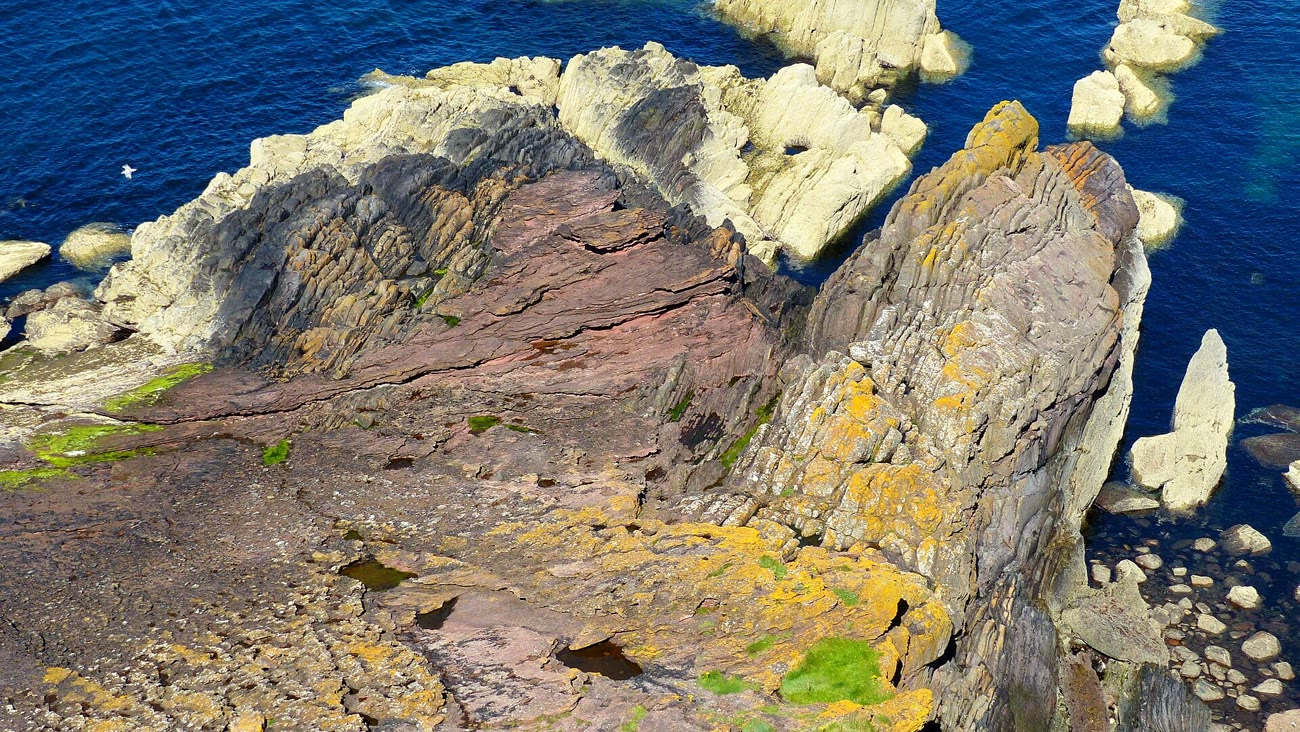
\includegraphics[width=0.7\linewidth]{images/book3/b1-siccar-point.jpg}

{\small A \omterm{def:b1:cross-sections:unconformity}{discordância} de Hutton em Siccar Point: camadas cinzentas, siluriana, quase verticais embaixo; camadas vermelhas devonianas inclinadas suavemente em cima. Fotografia PawełS, CC BY-SA 4.0 (Wikimedia Commons).}
% ledger: commons:siccar-point
\end{center}
\end{history}

\begin{inthefield}[Geologia para um túnel]
\begin{minipage}[t]{0.6\linewidth}\vspace{0pt}
Antes de um túnel ser projetado, os geólogos de engenharia traçam seções ao longo da sua linha a partir do \omterm{def:b1:geological-maps:geological-map}{mapa geológico}, de sondagens perfuradas em intervalos ao longo do traçado e de levantamentos geofísicos. Eles preveem cada unidade que o túnel vai cortar, as falhas que ele vai cruzar e onde a água pode entrar. Durante a perfuração, os geólogos da empreiteira registram a rocha exposta na frente a cada avanço, comparam-na com a previsão e atualizam a seção; sondagens de avanço perfuradas à frente da máquina testam o terreno antes que ela o alcance, sobretudo perto de uma falha prevista ou em calcário que pode conter cavidades. Uma zona de falha de rocha triturada é um perigo clássico, tanto mais quando a mesma rocha ocorre dos dois lados e nada na frente avisa dela.
\end{minipage}\hfill
\begin{minipage}[t]{0.37\linewidth}\vspace{0pt}
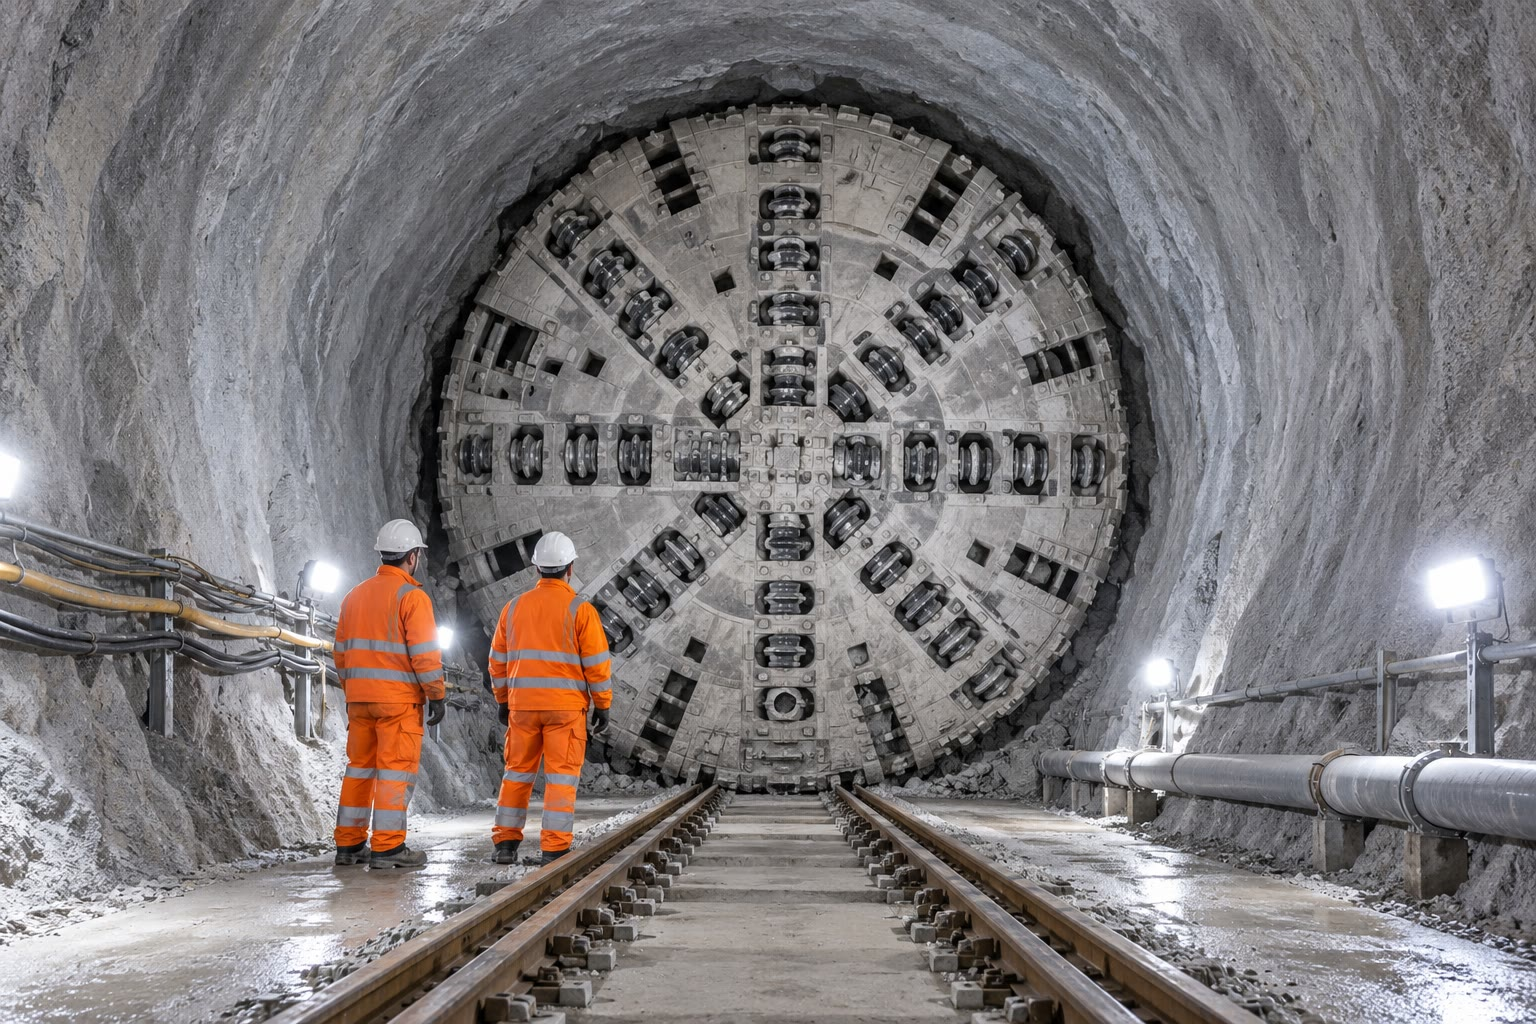
\includegraphics[width=\linewidth]{images/book3/ai/b1-tunnel-boring.jpg}
\end{minipage}
\end{inthefield}

\section{Exercícios}

\begin{exercise}[$\star$]\label{exo:b1:cross-sections:1}
Uma seção é desenhada a partir de um mapa na escala 1:25\,000, com escala vertical de \qty{1}{cm} para \qty{100}{m}. Qual é o seu \omterm{def:b1:cross-sections:section}{exagero vertical}?
\end{exercise}

\begin{exercise}[$\star$]\label{exo:b1:cross-sections:2}
Uma camada mergulha \ang{40} para \ang{090}. Qual é o seu \omterm{def:b1:cross-sections:apparent-dip}{mergulho aparente} em uma seção vertical de \omterm{def:b1:spherical-astronomy:horizontal}{azimute} \ang{060}? E de \omterm{def:b1:spherical-astronomy:horizontal}{azimute} \ang{000}?
\end{exercise}

\begin{exercise}[$\star$]\label{exo:b1:cross-sections:3}
Um furo de sondagem vertical atravessa \qty{120}{m} de arenito cujas camadas mergulham \ang{12.16}. Qual é a \omterm{def:b1:cross-sections:thickness}{espessura verdadeira} do arenito?
\end{exercise}

\begin{exercise}[$\star$]\label{exo:b1:cross-sections:4}
Um contato que mergulha \ang{12} no plano de uma seção é desenhado com exageros verticais de 2, 3 e 5. Em que ângulos ele aparece?
\end{exercise}

\begin{exercise}[$\star\star$]\label{exo:b1:cross-sections:5}
Uma camada mergulha \ang{25}. Seu \omterm{def:b1:geological-maps:geological-map}{afloramento} tem \qty{300}{m} de largura, medida perpendicularmente à \omterm{def:b1:geological-maps:attitude}{direção}. Calcule a sua \omterm{def:b1:cross-sections:thickness}{espessura verdadeira} (a) em terreno plano; (b) em terreno inclinado de \ang{10} no sentido oposto ao do \omterm{def:b1:geological-maps:attitude}{mergulho}, sendo a largura medida ao longo do terreno; (c) em terreno inclinado de \ang{10} no mesmo sentido do \omterm{def:b1:geological-maps:attitude}{mergulho}.
\end{exercise}

\begin{exercise}[$\star\star$]\label{exo:b1:cross-sections:6}
Uma camada mostra um \omterm{def:b1:cross-sections:apparent-dip}{mergulho aparente} de \ang{20} para o norte em uma seção norte--sul, e de \ang{30} para leste em uma seção leste--oeste. Encontre o seu \omterm{def:b1:geological-maps:attitude}{sentido de mergulho} e o seu \omterm{def:b1:geological-maps:attitude}{mergulho} verdadeiro.
\end{exercise}

\begin{exercise}[$\star\star$]\label{exo:b1:cross-sections:7}
A base do calcário no flanco leste mergulha \ang{12.16}. Qual é o espaçamento horizontal das suas \omterm{def:b1:cross-sections:structure-contour}{curvas estruturais} traçadas a cada \qty{100}{m}? Confira no \omterm{def:b1:cross-sections:structure-contour}{mapa de curvas estruturais}.
\end{exercise}

\begin{exercise}[$\star\star$]\label{exo:b1:cross-sections:8}
A partir da tabela das sondagens, calcule a altitude da base do folhelho em B1 e em B3. Sobre B2 o folhelho foi erodido: a partir da \omterm{def:b1:cross-sections:thickness}{espessura vertical} do calcário, encontre a altitude que a sua base teria ali, e o \omterm{def:b1:cross-sections:apparent-dip}{mergulho aparente} desse contato entre B1 e B2 na seção C--D. O que a comparação entre B1 e B3 diz sobre a \omterm{def:b1:geological-maps:fold}{dobra}?
\end{exercise}

\begin{exercise}[$\star\star$]\label{exo:b1:cross-sections:9}
Uma falha normal que mergulha \ang{50} para \ang{180} tem um \omterm{def:b1:cross-sections:throw}{rejeito} de \qty{150}{m}. Calcule o seu \omterm{def:b1:cross-sections:throw}{afastamento horizontal}. Em uma seção vertical de \omterm{def:b1:spherical-astronomy:horizontal}{azimute} \ang{150}, quais são o \omterm{def:b1:cross-sections:apparent-dip}{mergulho aparente} da falha e a separação dos dois cortes de uma camada horizontal ao longo da seção?
\end{exercise}

\begin{exercise}[$\star\star\star$]\label{exo:b1:cross-sections:10}
Para uma camada que mergulha \ang{40}, em quais direções de seção o \omterm{def:b1:cross-sections:apparent-dip}{mergulho aparente} é a metade do \omterm{def:b1:geological-maps:attitude}{mergulho} verdadeiro, isto é, \ang{20}? Mostre que o \omterm{def:b1:cross-sections:apparent-dip}{mergulho aparente} varia pouco perto da \omterm{def:b1:geological-maps:attitude}{direção} do \omterm{def:b1:geological-maps:attitude}{mergulho} e depressa perto da \omterm{def:b1:geological-maps:attitude}{direção} da linha de \omterm{def:b1:geological-maps:attitude}{direção}.
\end{exercise}

\begin{exercise}[$\star\star\star$]\label{exo:b1:cross-sections:11}
Um furo de sondagem atravessa o calcário do flanco leste (\omterm{def:b1:cross-sections:thickness}{espessura verdadeira} \qty{176.0}{m}, \omterm{def:b1:geological-maps:attitude}{mergulho} \ang{12.16} para \ang{080.7}). Que comprimento de testemunho ele recupera (a) se for vertical; (b) se for inclinado de \ang{60} abaixo da horizontal para \ang{260.7}; (c) inclinado de \ang{60} para \ang{080.7}? (Sugestão: o comprimento é $t/\cos\psi$, em que $\psi$ é o ângulo entre o furo e a normal ao acamamento.)
\end{exercise}

\begin{exercise}[$\star\star\star$]\label{exo:b1:cross-sections:12}
Em uma \omterm{def:b1:cross-sections:unconformity}{discordância angular}, as camadas inferiores mergulham \ang{70} para \ang{090} e as superiores mergulham \ang{20} para \ang{270}, com a mesma \omterm{def:b1:geological-maps:attitude}{direção}. Gire todo o \omterm{def:b1:geological-maps:geological-map}{afloramento} em torno da \omterm{def:b1:geological-maps:attitude}{direção} para trazer as camadas superiores de volta à horizontal: qual era o \omterm{def:b1:geological-maps:attitude}{mergulho} das camadas inferiores quando as superiores foram depositadas? Escreva a história do \omterm{def:b1:geological-maps:geological-map}{afloramento} em ordem.
\end{exercise}

\section{Problema: um túnel sob as Colinas de Varden}

\begin{problem}[{Problema de fim de semana --- quais rochas um túnel vai cortar, onde ele encontrará a falha e quanto calcário ele vai perfurar}]
\label{pb:b1:cross-sections:1}
% numbers from figdata/bachelor-1/varden_sections.py (model region.py) and the scratch calculator
O túnel corre exatamente para leste ao longo da linha C--D ($y = \qty{6}{km}$), em altitude constante de \qty{200}{m}, de $x = \qty{1}{km}$ até $x =
\qty{9}{km}$. A altitude do terreno ao longo de C--D, a cada quilômetro a partir de $x = 0$, é:
\begin{center}
\small
\begin{tabular}{lccccccccccc}
\hline
$x$ (km) & 0 & 1 & 2 & 3 & 4 & 5 & 6 & 7 & 8 & 9 & 10 \\
$z$ (m) & 509 & 556 & 467 & 370 & 435 & 534 & 501 & 455 & 406 & 339 & 405 \\
\hline
\end{tabular}
\end{center}
Use a tabela de sondagens do capítulo, a seção C--D desenhada com $e = 3$, a \omterm{def:b1:geological-maps:attitude}{atitude} do flanco leste (\omterm{def:b1:geological-maps:attitude}{mergulho} \ang{12.16} para \ang{080.7}; o flanco oeste é a sua imagem especular, mergulhando para \ang{279.3}), e a falha normal, que mergulha \ang{60} para \ang{120}, tem \omterm{def:b1:cross-sections:throw}{rejeito} de \qty{200}{m} e passa pelo ponto $x = \qty{4.30}{km}$, $y = \qty{1.00}{km}$,
$z = \qty{250}{m}$.

\medskip
\noindent\textbf{Parte I --- O perfil e as unidades.}
\begin{enumerate}
  \item Quais são as maiores e as menores espessuras de rocha acima do túnel nos pontos quilométricos entre $x = 1$ e $x = 9$?
  \item Na seção impressa, \qty{1}{km} de distância horizontal mede \qty{1.4}{cm} e \qty{1}{km} de altitude mede \qty{4.2}{cm}. Confira que $e = 3$.
  \item A partir do perfil de B2, encontre a altitude da base do arenito na crista do \omterm{def:b1:geological-maps:fold}{anticlinal}.
  \item Em qual unidade está o túnel em $x = \qty{3.5}{km}$?
  \item Calcule a altitude da base do calcário em B1 e em B3.
  \item A partir da seção, liste em ordem as unidades que o túnel atravessa de $x = 1$ até $x = \qty{9}{km}$.
\end{enumerate}

\medskip
\noindent\textbf{Parte II --- Mergulhos na seção.}
\begin{enumerate}[resume]
  \item Calcule o \omterm{def:b1:cross-sections:apparent-dip}{mergulho aparente} do flanco leste em C--D a partir da sua \omterm{def:b1:geological-maps:attitude}{atitude}.
  \item Confira-o a partir das altitudes da base do calcário em B2 e B3.
  \item Em que ângulo o flanco leste é desenhado na seção com $e = 3$?
  \item Calcule o \omterm{def:b1:cross-sections:apparent-dip}{mergulho aparente} da falha em C--D.
  \item Por que o \omterm{def:b1:cross-sections:apparent-dip}{mergulho aparente} dos flancos em C--D fica tão próximo do seu \omterm{def:b1:geological-maps:attitude}{mergulho} verdadeiro, e o da falha, menos?
\end{enumerate}

\medskip
\noindent\textbf{Parte III --- A falha.}
\begin{enumerate}[resume]
  \item Mostre que, no plano $y = \qty{6}{km}$, a falha está em
        \[ x = 4300 + \frac{2500 - (z - 250)\tan\ang{30}}{\sin\ang{120}}
           \quad\text{(metros)}. \]
  \item Onde o túnel encontra a falha?
  \item Calcule o \omterm{def:b1:cross-sections:throw}{afastamento horizontal} da falha e a separação dos dois cortes de um contato ao longo de C--D.
  \item Qual bloco está abatido, e qual unidade está no nível do túnel de cada lado da falha?
  \item Por que a falha é um perigo que a equipe de perfuração não poderia ver chegando a partir da rocha na frente? Como os engenheiros se protegem contra ela?
\end{enumerate}

\medskip
\noindent\textbf{Parte IV --- O calcário.}
\begin{enumerate}[resume]
  \item Qual é a \omterm{def:b1:cross-sections:thickness}{espessura vertical} do calcário em B1?
  \item Qual é a sua \omterm{def:b1:cross-sections:thickness}{espessura verdadeira}?
  \item Mostre que, a oeste da falha em C--D, a base do arenito está
        em
        \[ z_b = 160.16 - |x - 3500|\tan\ang{12.0} \quad\text{(metros)}. \]
  \item O túnel está no calcário quando a sua base fica abaixo de \qty{200}{m} e o seu topo, acima. Mostre que isso acontece para $377.1 < |x - 3500|
        < 1224.0$.
  \item Dê os quatro pontos em que o túnel entra e sai do calcário.
  \item Mostre que o comprimento perfurado em cada flanco é $h/\tan\beta$, em que $h$ é a \omterm{def:b1:cross-sections:thickness}{espessura vertical} e $\beta$ o \omterm{def:b1:cross-sections:apparent-dip}{mergulho aparente}, e calcule-o.
  \item Qual é o comprimento total de calcário que o túnel perfura?
\end{enumerate}
\end{problem}
